\chapter{Communication and Data Handling}
\label{chap:comms}
%more detail: add exact system noise temperature calculation

\section{Space Mission Architecture and Downflowing Requirements}
%mission architecture
The communication architecture consists of three main elements: the aerobot in the Venus cloud layer, the Venus orbiter, and the ESTRACK ground station on Earth. The aerobot collects science and housekeeping data and sends it to the orbiter through a short-range relay link. The orbiter then stores and forwards the data to Earth using a deep-space communication link.

The same relay architecture is used for command uplink in the opposite direction: commands are sent from Earth to the orbiter and then relayed to the aerobot for mode updates, sampling changes, data-handling updates, and contingency operations. Direct aerobot--Earth communication is not selected, because the large Earth--Venus distance would require transmitter power, antenna gain, and pointing accuracy that are not practical for a balloon-borne gondola.

%requirements 
\medskip
\noindent A set of top-level communication requirements is defined in Table~\ref{tab:communication_requirements}. 
% These requirements are used to guide the communication system trade-off and to ensure that both the aerobot-orbiter relay link and the orbiter-Earth deep-space link satisfy the mission needs.

\begin{table}[H]
    \centering
    \small
    \caption{Top-level communication requirements.}
    \label{tab:communication_requirements}
    \begin{tabular}{p{0.13\textwidth} p{0.33\textwidth} p{0.44\textwidth}}
        \hline
        \textbf{ID} & \textbf{Requirement} & \textbf{Rationale} \\
        \hline
        REQ-COM-01 & 
        The bit error rate of the data received on Earth shall not exceed 
        $1 \times 10^{-6}$. & 
        This value is selected in accordance with ITU recommendations for 
        unmanned deep-space research missions~\cite{ITU-R-SA1014-4-2023}. \\
        \hline
        REQ-COM-02 & 
        The communication link from the aerobot to the orbiter shall support a useful data rate of at least $1500~\mathrm{bit/s}$. & 
        This requirement is derived mission description \\
        \hline
        REQ-COM-03 & 
        The communication link between the orbiter and Earth shall be compatible with the ESTRACK ground-station network. & 
        Compatibility with ESTRACK constrains the selection of frequency band, modulation, coding, antenna gain, and operational link budget. \\
        \hline
        REQ-COM-04 &
        Each communication link shall close with a positive link margin under worst-case mission geometry. &
        This ensures reliable communication at maximum range, including losses due to free-space propagation, atmosphere, pointing, polarization mismatch, and implementation losses. \\
        \hline
        REQ-COM-05 & The antenna shall maintain a communication link with the orbiter for >90\% of the time whenever the orbiter is above the local horizon & Maintaining communication over the visibility window maximizes the available time for data transmission and reduces the risk of data loss. NASA/JPL’s DESCANSO link design material states that historical deep-space RF links have achieved an overall link availability of about 90\%  \cite{chen2006linkSystemDesign} \\
        \hline
    \end{tabular}
\end{table}


\section{Frequency band selection}
The frequency band selection is a key design driver because it affects achievable data rate, antenna gain, transmitter power, link margin, propagation losses, ground-station compatibility, and frequency-allocation constraints. For the orbiter--Earth link, the main ESTRACK-compatible deep-space options are S-band, X-band, and Ka-band, as summarized in \autoref{tab:estrack_frequency_bands}. X-band is selected as the baseline because it provides the best compromise between reliability, data-rate capability, antenna size, and ESTRACK compatibility. Compared with S-band, it offers higher bandwidth and higher antenna gain for a given antenna size; compared with Ka-band, it is less sensitive to atmospheric attenuation, rain losses, and pointing errors, making it more robust for a relatively low-data-rate Venus mission.

\begin{table}[H]
    \centering
    \small
    \caption{Candidate ESTRACK-compatible frequency bands for the orbiter--Earth link.}
    \label{tab:estrack_frequency_bands}
    \begin{tabular}{p{0.22\textwidth} p{0.34\textwidth} p{0.34\textwidth}}
        \hline
        \textbf{Band} & \textbf{Uplink: Earth to orbiter} & \textbf{Downlink: orbiter to Earth} \\
        \hline
        S-band & $2110$--$2120~\mathrm{MHz}$ & $2290$--$2300~\mathrm{MHz}$ \\
        \hline
        X-band & $7145$--$7190~\mathrm{MHz}$ & $8400$--$8450~\mathrm{MHz}$ \\
        \hline
        Ka-band & $34.2$--$34.7~\mathrm{GHz}$ & $31.8$--$32.3~\mathrm{GHz}$ \\
        \hline
    \end{tabular}
\end{table}

For the aerobot--orbiter relay link, direct use of X-, S-, or Ka-band is less attractive because the balloon gondola has limited pointing capability and power. The candidate proximity-link bands are therefore VHF, UHF, and S-band, as shown in \autoref{tab:aerobot_orbiter_frequency_bands}. VHF has low path loss and is robust, but requires larger antennas and has less modern planetary relay heritage. S-band is possible, but has higher path loss and generally requires better antenna gain or pointing. UHF is selected as the baseline because it is well suited to short-range planetary relay, low data rates, low spacecraft complexity, broad antenna coverage, and weak pointing requirements.

\begin{table}[H]
    \centering
    \small
    \caption{Candidate frequency bands for the aerobot--orbiter communication link.}
    \label{tab:aerobot_orbiter_frequency_bands}
    \begin{tabular}{p{0.30\textwidth} p{0.50\textwidth}}
        \hline
        \textbf{Band} & \textbf{Frequency range} \\
        \hline
        VHF & $30$--$300~\mathrm{MHz}$ \\
        \hline
        UHF & $300~\mathrm{MHz}$--$3~\mathrm{GHz}$ \\
        \hline
        S-band & $2$--$4~\mathrm{GHz}$ \\
        \hline
    \end{tabular}
\end{table}

\section{Link Analysis}
\subsection{Modulation, Coding and Spectral Efficiency}
Based on the modulation trade-off in \autoref{tab:modulation_tradeoff}, the most suitable schemes for the aerobot--orbiter UHF link are BPSK, MSK/GMSK, and QPSK. Since the required data rate is low, robustness and power efficiency are more important than spectral efficiency. BPSK is power-efficient and requires a low \(E_b/N_0\), reducing transmitter power, but it requires coherent carrier recovery and is therefore sensitive to Doppler, oscillator stability, and phase tracking. MSK/GMSK is retained as the main alternative because its constant-envelope waveform allows efficient nonlinear power amplification and good spectral containment. QPSK is possible, but its higher spectral efficiency is not necessary for this low-rate link, while FSK and higher-order PSK/QAM schemes are rejected due to lower power efficiency or higher sensitivity to noise, phase errors, and amplifier nonlinearities.

\begin{table}[H]
    \centering
    \small
    \caption{Comparison of candidate modulation schemes}
    \label{tab:modulation_tradeoff}
    \begin{tabularx}{\textwidth}{p{0.18\textwidth} X X}
        \toprule
        \textbf{Modulation} & \textbf{Main advantage} & \textbf{Main disadvantage} \\
        \midrule
        Noncoherent BFSK & Simple and robust acquisition without coherent carrier recovery. & Higher required \(E_b/N_0\) and larger bandwidth than BPSK. \\
        \midrule
        Coherent BFSK & More energy-efficient than noncoherent BFSK. & Still less efficient than BPSK and requires coherent reception. \\
        \midrule
        BPSK & Very power-efficient and robust for low-rate links. & Requires coherent carrier recovery and phase tracking. \\
        \midrule
        MSK/GMSK & Constant-envelope waveform enables efficient power amplification and good spectral containment. & Slightly more complex than simple FSK and requires compatible modem implementation. \\
        \midrule
        QPSK & Higher spectral efficiency than BPSK with similar ideal \(E_b/N_0\) performance. & Extra spectral efficiency is not needed and phase recovery is more complex. \\
        \midrule
        8-PSK / 16-PSK & Higher spectral efficiency. & Requires higher \(E_b/N_0\) and is more sensitive to phase noise and nonlinearities. \\
        \midrule
        16-QAM & High spectral efficiency using amplitude and phase. & Requires high SNR, accurate amplitude/phase tracking, and a linear power amplifier. \\
        \bottomrule
    \end{tabularx}
\end{table}

\begin{figure}[H]
    \centering

    \begin{minipage}[t]{0.48\textwidth}
        \vspace{0pt}
        \small
        Channel coding is included to improve link reliability by adding redundancy, allowing the receiver to detect and correct bit errors after demodulation. This reduces the required \(E_b/N_0\) for a given BER and is included in the link budget as coding gain, at the cost of transmitting additional non-information bits. Candidate schemes include convolutional coding with Viterbi decoding, Turbo coding, and LDPC coding, with approximate coding gains shown in \autoref{fig:coding-gains}. For the aerobot--orbiter link, decoding is mainly performed on the orbiter. Pulse shaping is defined by the raised-cosine roll-off factor, which reduces intersymbol interference but increases occupied bandwidth.
    \end{minipage}
    \hfill
    \begin{minipage}[t]{0.48\textwidth}
        \vspace{0pt}
        \centering
        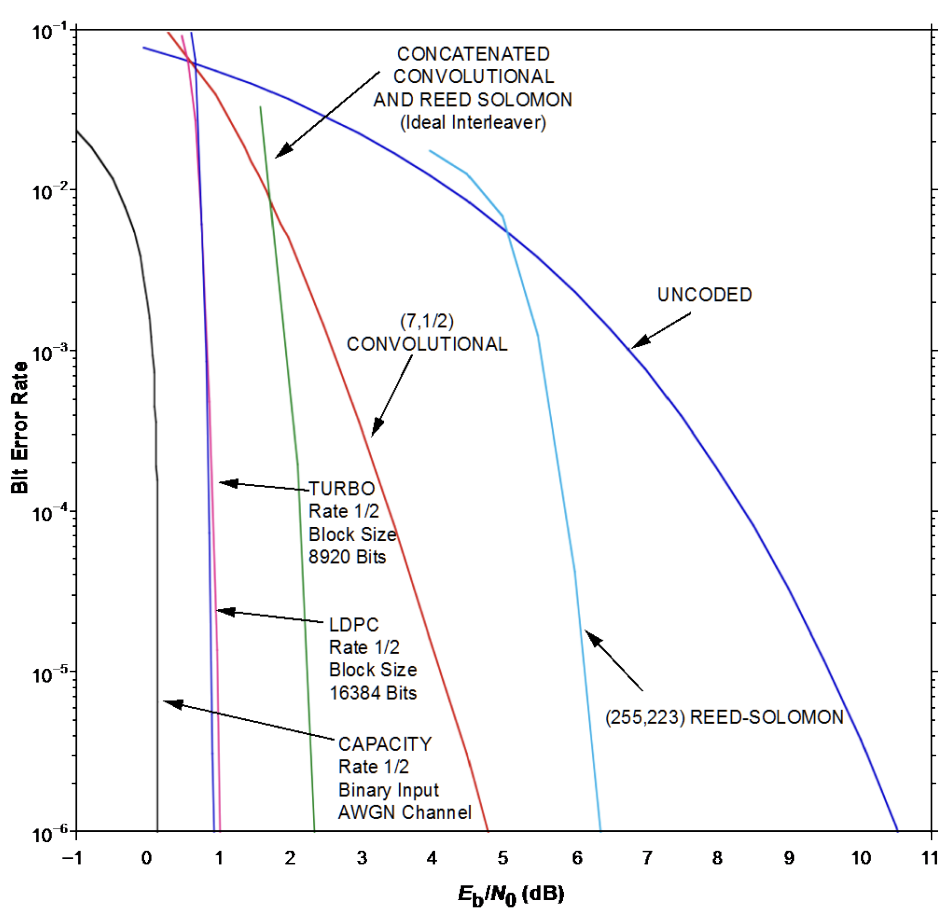
\includegraphics[width=\linewidth]{fig/Coding gains.png}
        \caption{Performance comparison of selected convolutional, Reed--Solomon, concatenated, LDPC, and Turbo codes \cite{ccsds2020_tm_sync_channel_coding}.}
        \label{fig:coding-gains}
    \end{minipage}

\end{figure}
\subsection{Propagation losses}
The simplest source of propagation loss is the free-space path loss, which represents the spreading loss of an electromagnetic wave as it propagates through space. It is given by \autoref{eq:space-loss}

\begin{equation}
    L_{fs} = 20 \log_{10}\left(\frac{4 \pi d}{\lambda}\right)
    \label{eq:space-loss}
\end{equation}

\noindent where $L_{fs}$ is the free-space path loss in dB, $d$ is the distance between the transmitter and receiver, and $\lambda$ is the signal wavelength.

\medskip
\noindent The second source of signal loss is absorption by atmospheric gases. The atmosphere of Venus consists of approximately 96.5\% $CO_2$ and 3.5\% $N_2$. \autoref{fig:absorption-rates} shows the absorption rates, expressed in dB/km, of several gases in the Venusian atmosphere for X-band and S-band frequencies. The figure also shows that below altitudes of approximately 50 km, the abundance of $H_2SO_4$ becomes significant, extending down to about 30 km. At lower frequencies, such as those in the UHF range, these absorption rates are expected to be even lower.

\begin{figure}[H]
    \centering

    \begin{minipage}{0.48\textwidth}
        \centering
        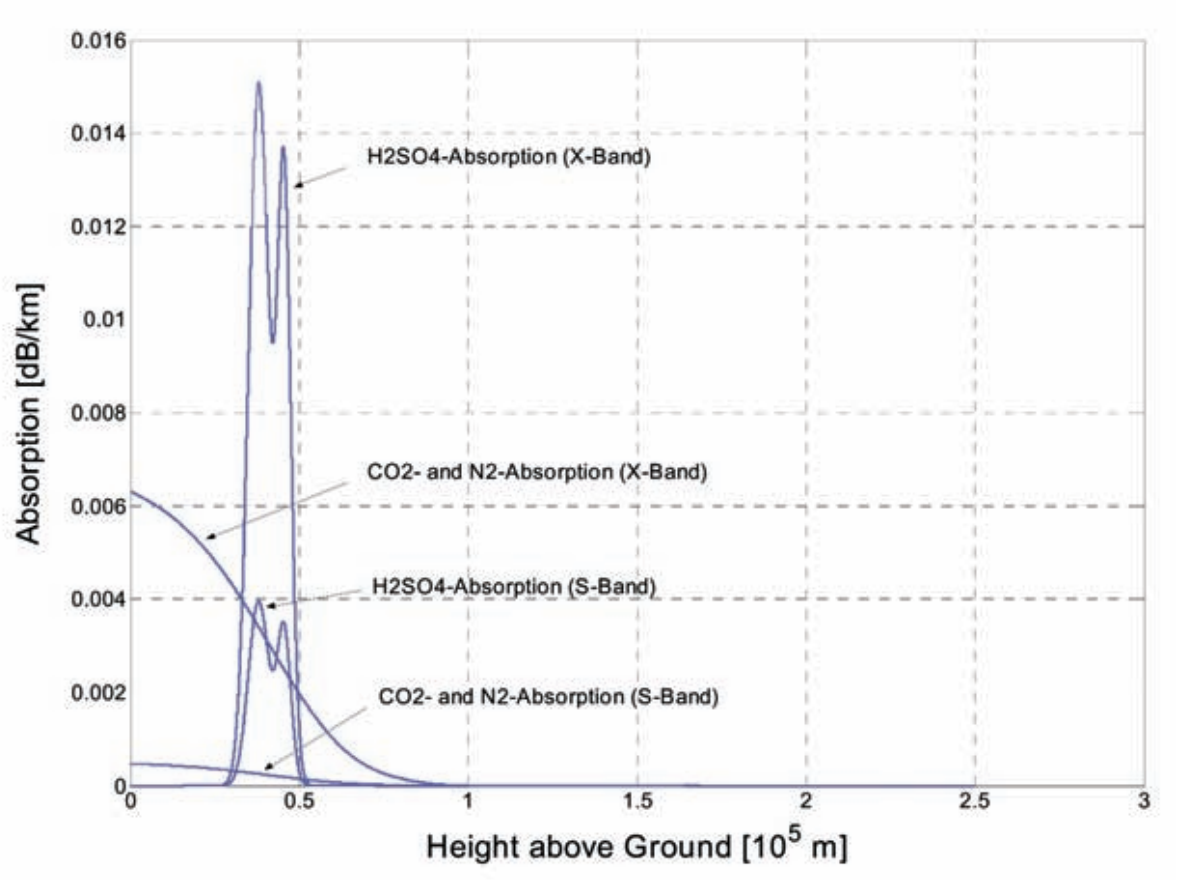
\includegraphics[width=\linewidth]{fig/Radio absorption Venus Atmosphere gasses.png}
        \caption{Average absorption profile as a function of altitude for $H_2SO_4(g)$, $CO_2$, and $N_2$ in the atmosphere of Venus \cite{hausler2007vera}.}
        \label{fig:absorption-rates}
    \end{minipage}
    \hfill
    \begin{minipage}{0.48\textwidth}
        \centering
        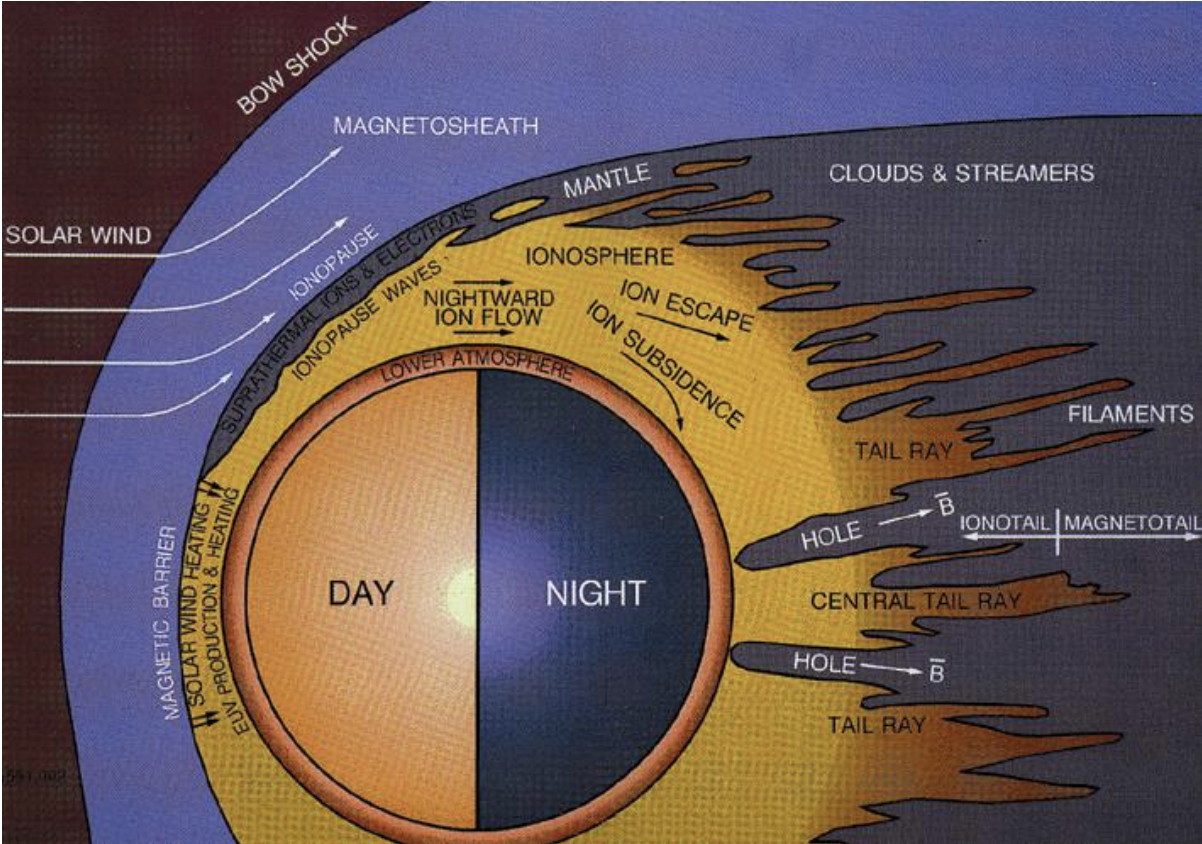
\includegraphics[width=\linewidth]{fig/Ionosphere.png}
        \caption{A sketch of the most important plasma boundaries and interaction regions in the environment of Venus \cite{angsmann2011magnetic}.}
        \label{fig:ionosphere illustation}
    \end{minipage}

\end{figure}

The Venus ionosphere is dynamic because electron density varies with altitude, solar illumination, solar activity, and solar-wind conditions. Since Venus lacks a strong intrinsic magnetic field, its plasma environment is mainly shaped by interaction with the solar wind, forming an induced magnetosphere as illustrated in \autoref{fig:ionosphere illustation}. These variations can affect UHF propagation between the aerobot and orbiter and are therefore included in the link-budget loss model.

% \autoref{fig:electron-density} shows the variation of electron density with time and solar zenith angle. 
For the link budget, a conservative case is used by taking the maximum electron-density envelope and the highest ionopause condition. The ionospheric absorption loss is calculated as
\begin{equation}
L_{\mathrm{ion,abs}} =
\frac{1.17 \times 10^{-6}\,\nu\,\mathrm{TEC}}
{n_{\mathrm{re}} f^2}
\label{eq:ionosphere-absorption}
\end{equation}
where \(L_{\mathrm{ion,abs}}\) is the absorption loss in dB, \(\nu\) is the effective electron collision frequency, \(f\) is the signal frequency, and \(n_{\mathrm{re}}\) is the real part of the plasma refractive index. For UHF, \(n_{\mathrm{re}}\approx 1\), since the signal frequency is much larger than the local plasma frequency.

% \begin{figure}[ht]
%     \centering

%     \begin{subfigure}[t]{0.48\linewidth}
%         \centering
%         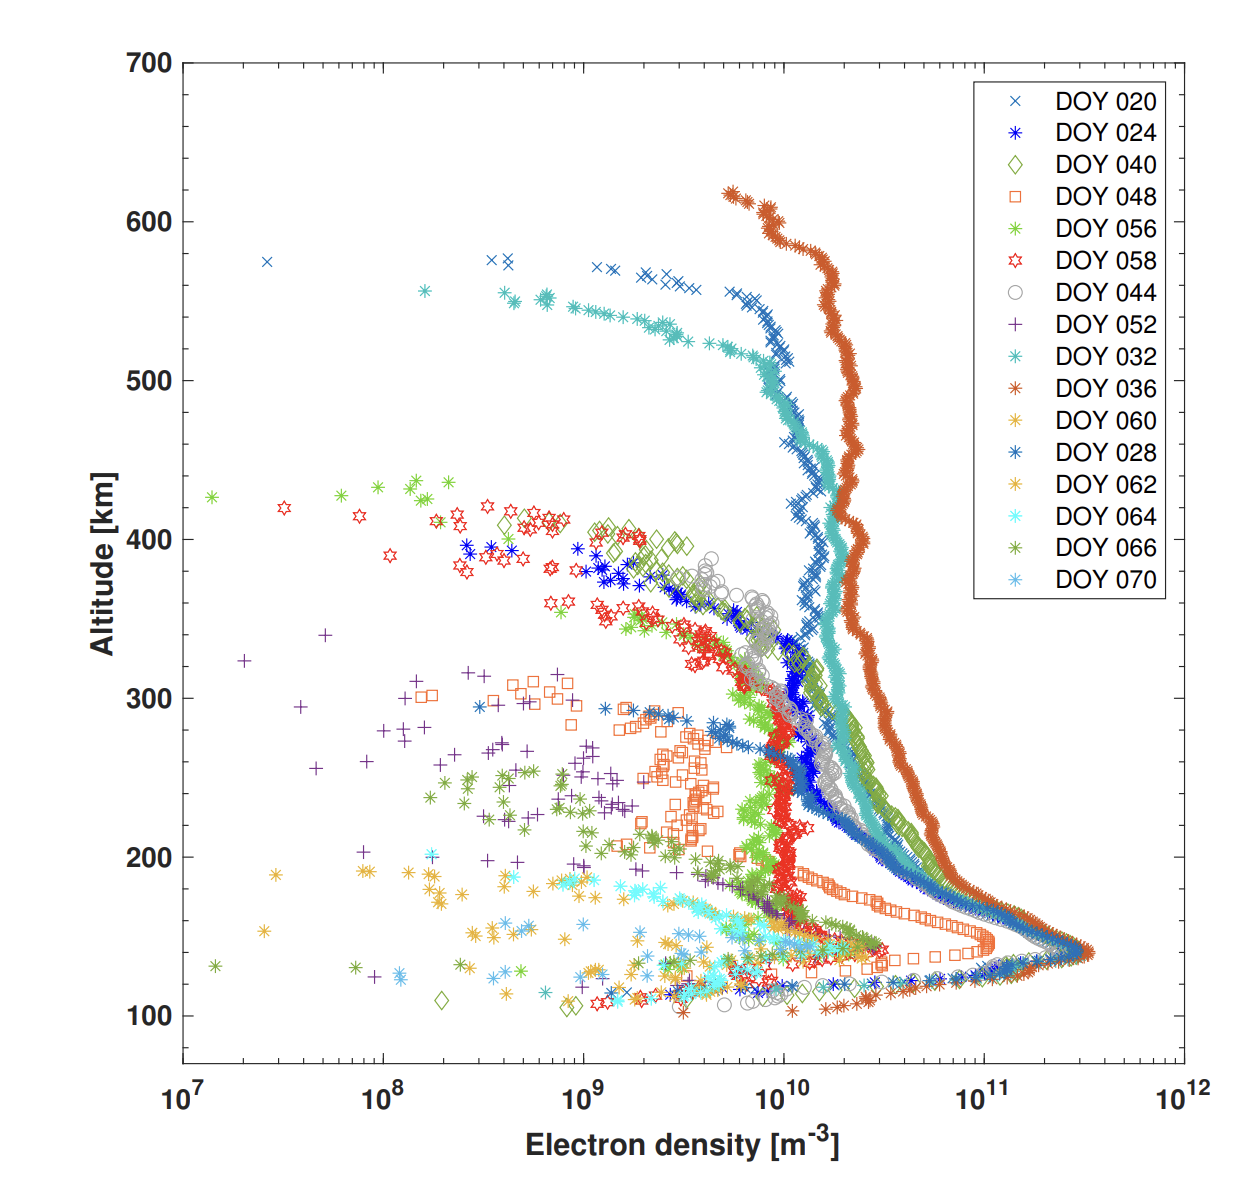
\includegraphics[width=\linewidth]{fig/Electron density different moments.png}
%         \caption{Electron density measured at different time instances}
%         \label{fig:electron-density-1}
%     \end{subfigure}
%     \hfill
%     \begin{subfigure}[t]{0.48\linewidth}
%         \centering
%         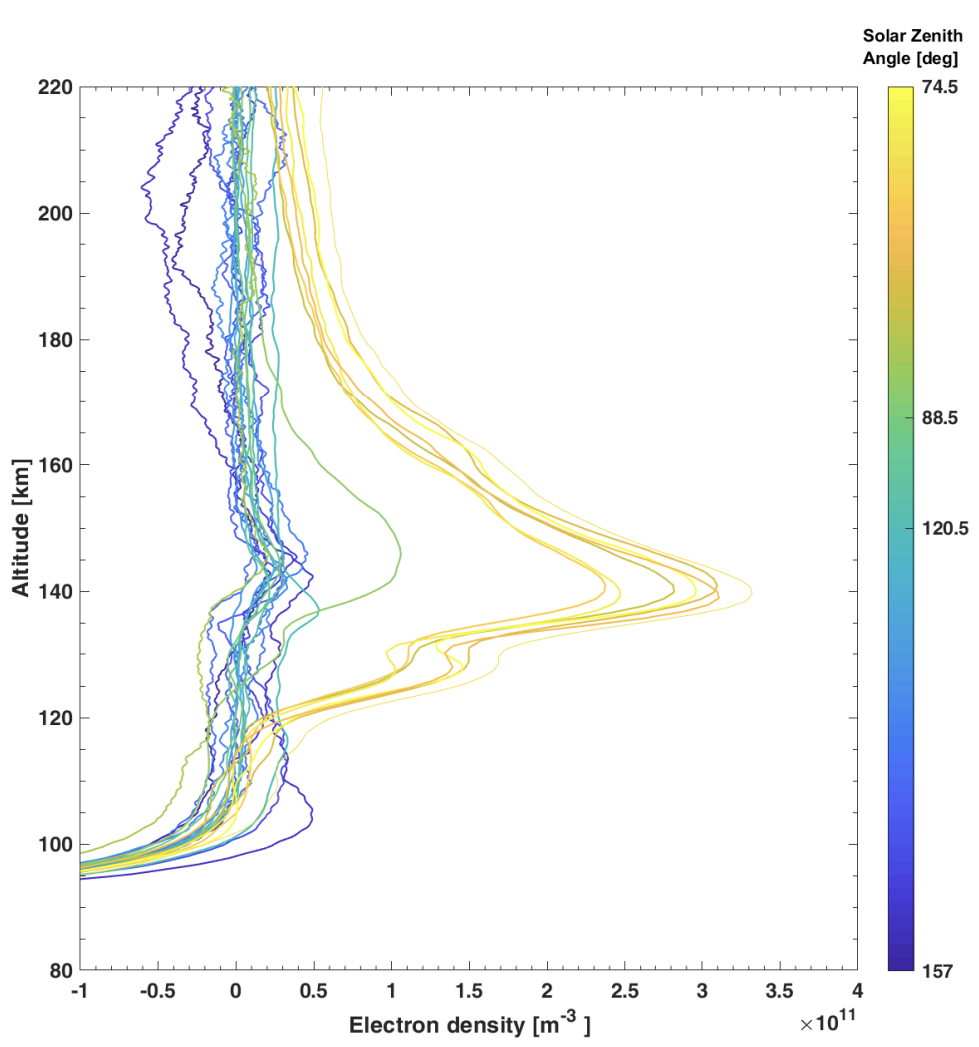
\includegraphics[width=\linewidth]{fig/electron density solar.png}
%         \caption{Electron density measured for different solar zenith angles}
%         \label{fig:electron-density-2}
%     \end{subfigure}

    \caption{Electron density vs. altitude: (a) at different time instances and (b) for different solar zenith angles \cite{gramigna2023venus}.}
    \label{fig:electron-density}
\end{figure}

The total electron content along the path is
\begin{equation}
\mathrm{TEC} = \int_{\text{path}} N_e(s)\, ds
\label{eq:TEC}
\end{equation}
where \(N_e(s)\) is the electron density along the signal path. A numerical tool was used to evaluate atmospheric and ionospheric losses for different elevation angles and altitudes, including the lowest operational altitude of \(52~\mathrm{km}\). Combining the conservative ionospheric model with atmospheric gas and cloud losses gives a maximum total propagation loss of \(L_{\mathrm{gasses,ionosphere}} = 2.5~\mathrm{dB}\), which is used in the UHF link budget.

\medskip
% \noindent A separate rain attenuation term is not included in the link budget. Although sulfuric-acid droplets may fall through the Venusian cloud layer, their effect is already covered by the atmospheric/cloud attenuation term for $\mathrm{H_2SO_4}$ aerosols and droplets. At UHF, the signal wavelength is much larger than the expected droplet size, so additional attenuation due specifically to precipitation is assumed to be small and is included within the atmospheric-loss uncertainty and link margin.
% add this text for clarity later
%Faraday rotation, group delay, phase advance(= average/total phase shift due to TEC, while Phase scintillation = rapid variation of that phase shift due to changing TEC), and Doppler-like ionospheric effects must be analyzed under polarization, synchronization, and receiver tracking requirement
%reflection and diffraction effect can be ignored for line of sight com
%scattering included in db/km of cloud/atmospheric attenuation
\medskip
\noindent Scintillation is not treated as a fixed atmospheric attenuation, but as a fade margin. 
% Since the aerobot-orbiter link operates at UHF, ionospheric scintillation may cause  short-term amplitude and phase fluctuations, especially at low elevation angles where the slant path through the atmosphere and ionosphere is longest. 
Therefore a 2 dB fading margin is incorporated in accordance with SMAD\cite{wertz1999smad}.
%note: Scintillation is not an average attenuation loss.
%It is a temporary fluctuation in received power and phase.
The total atmospheric attenuation due to the earth is given to be $0.3dB$ for operational conditions, and $0.5 dB$ in case of moderate rain\cite{brizzolari2024dsa4attenuation}. 
\subsection{antenna options}

The aerobot operates at UHF and has limited attitude control, so the antenna must provide broad, non-directional coverage rather than high directivity. Wire antennas are therefore the most suitable class because they are simple, lightweight, mechanically robust, and easier to integrate on a balloon gondola. Printed antennas are possible but become relatively large at UHF, while array and aperture antennas are rejected because they add complexity, pointing requirements, mass, and power demand. A two-antenna configuration is selected, with antennas placed near opposite top edges of the gondola to improve low-elevation visibility, reduce blockage during gondola tilt, and relax attitude-control requirements.

The antenna trade-off in \autoref{tab:antenna_tradeoff} assumes that local reflectors or large backplanes are avoided. Although these could reduce radiation toward Venus, they would also make the antenna pattern more directional and could degrade the low-elevation coverage needed during orbiter passes.

% \begingroup
% \scriptsize
% \renewcommand{\arraystretch}{1.18}
% \setlength{\tabcolsep}{2pt}

% \begin{longtable}{|p{0.045\textwidth}|p{0.115\textwidth}|p{0.17\textwidth}|p{0.13\textwidth}|p{0.13\textwidth}|p{0.12\textwidth}|p{0.105\textwidth}|p{0.11\textwidth}|p{0.1\textwidth}|}
% \caption{Scored feasible antenna type trade-off for the aerobot.}
% \label{tab:antenna_tradeoff} \\
% \hline
% \textbf{ID} &
% \textbf{Option$\downarrow$ / Criteria$\rightarrow$} &
% \textbf{Coverage / Visibility (30\%)} &
% \textbf{Gain Performance (5\%)} &
% \textbf{Pointing Loss Performance (25\%)} &
% \textbf{Polarization Loss Performance (15\%)} &
% \textbf{Mass / Integration (10\%)} &
% \textbf{Reliability (15\%)} &
% \textbf{Weighted score} \\
% \hline
% \endfirsthead

% \hline
% \textbf{ID} &
% \textbf{Option$\downarrow$ / Criteria$\rightarrow$} &
% \textbf{Coverage / Visibility (30\%)} &
% \textbf{Gain Performance (5\%)} &
% \textbf{Pointing Loss Performance (25\%)} &
% \textbf{Polarization Loss Performance (15\%)} &
% \textbf{Mass / Integration (10\%)} &
% \textbf{Reliability (15\%)} &
% \textbf{Weighted score} \\
% \hline
% \endhead

% \hline
% \multicolumn{9}{r}{\small Continued on next page} \\
% \endfoot

% \hline
% \endlastfoot

% ANT-1 &
% \textbf{Helical-ring / Huygens-source antenna\cite{morlaas2015helical}} &
% \cellcolor{score5!40}\textbf{5} -- Provides hemispherical coverage without requiring a large reflector as seen in \autoref{fig:helical-ring}, reducing radiation toward the Venus surface while maintaining broad useful coverage toward the orbiter. &
% \cellcolor{score4!40}\textbf{4} -- Moderate useful gain; the ideal Huygens-source pattern has a maximum directivity of about $4.77\,\mathrm{dBi}$, while still preserving broad angular coverage. &
% \cellcolor{score5!40}\textbf{5} -- Low pointing losses over the desired half-space due to the broad cardioid-like radiation pattern, making it attractive for a tilting or swinging gondola. &
% \cellcolor{score5!40}\textbf{5} -- Provides circular polarization over a wide angular region, reducing sensitivity to gondola rotation and polarization mismatch. &
% \cellcolor{score4!40}\textbf{4} -- Compact compared with reflector-backed solutions, but more complex to design, tune, feed, and manufacture than simple dipole-based antennas. &
% \cellcolor{score3!40}\textbf{3} -- Promising performance, but much lower heritage than crossed dipoles, monopoles, or quadrifilar helices. &
% \cellcolor{score5!40}\textbf{4.55} \\
% \hline

% ANT-2 &
% \textbf{Crossed drooping dipole} &
% \cellcolor{score4!40}\textbf{4} -- Provides improved low-elevation coverage compared with a standard crossed dipole, making it well suited for communication near the start and end of an orbiter pass. &
% \cellcolor{score3!40}\textbf{3} -- Still a low-gain antenna, but the drooped geometry directs more useful radiation toward lower elevation angles. &
% \cellcolor{score5!40}\textbf{5} -- Very good option for reducing pointing losses at low elevation angles, which are critical for maximizing the useful orbiter visibility window. &
% \cellcolor{score4!40}\textbf{4} -- Can provide circular polarization, reducing sensitivity to gondola rotation and polarization mismatch with the orbiter. &
% \cellcolor{score3!40}\textbf{3} -- More difficult to integrate than a standard crossed dipole because the drooped elements require additional clearance and mechanical support near the gondola edges. &
% \cellcolor{score5!40}\textbf{5} -- High reliability for non-pointed communication, especially when two antennas are placed on opposite top edges to reduce blockage and tilt sensitivity. &
% \cellcolor{score4!40}\textbf{4.25} \\
% \hline

% ANT-3 &
% \textbf{Quadrifilar helix} &
% \cellcolor{score4!40}\textbf{4} -- Provides broad upper-hemisphere coverage and circular polarization, making it suitable for communication with an orbiter over a wide range of gondola orientations. &
% \cellcolor{score3!40}\textbf{3} -- Low-to-moderate gain; generally better suited for wide coverage than high-gain communication. &
% \cellcolor{score4!40}\textbf{4} -- Pointing losses are low due to the broad radiation pattern, although low-elevation performance depends on the exact helix geometry. &
% \cellcolor{score5!40}\textbf{5} -- Naturally suited for circular polarization, reducing polarization mismatch during gondola rotation or swing. &
% \cellcolor{score2!40}\textbf{2} -- More bulky and mechanically complex than dipole-based options, especially at UHF frequencies. &
% \cellcolor{score4!40}\textbf{4} -- Good heritage for satellite-style communication, but the larger three-dimensional structure may be harder to protect and integrate on the gondola edge. &
% \cellcolor{score4!40}\textbf{3.90} \\
% \hline

% ANT-4 &
% \textbf{Crossed dipole / turnstile} &
% \cellcolor{score4!40}\textbf{4} -- Provides broad angular coverage, as seen in \autoref{fig:crossed-dipole}. With edge mounting, the gondola side may behave more like the reflector-influenced case, while the open side remains closer to the free-space case. &
% \cellcolor{score2!40}\textbf{2} -- Low-gain antenna; suitable for wide coverage, but the orbiter must provide sufficient receive sensitivity or antenna gain to close the link. &
% \cellcolor{score4!40}\textbf{4} -- Pointing losses are generally low due to the broad radiation pattern, but can increase near the horizon or in weak-pattern directions. &
% \cellcolor{score4!40}\textbf{4} -- Circular polarization reduces sensitivity to gondola rotation and can give near-zero polarization loss if the orbiter antenna has matching handedness. &
% \cellcolor{score5!40}\textbf{5} -- Low mass and simple integration; the radiating elements can be very lightweight at UHF frequencies. Each dipole is approximately $0.5\lambda$ long. &
% \cellcolor{score5!40}\textbf{5} -- Reliable, simple, and heritage-friendly, but it radiates more power into the undesired half-space than hemispherical antenna concepts. &
% \cellcolor{score4!40}\textbf{4.15} \\
% \hline

% ANT-5 &
% \textbf{Circularly polarized patch / crossed-slot patch} &
% \cellcolor{score2!40}\textbf{2} -- Provides good broadside upper-hemisphere coverage, but low-elevation coverage is poorer than for wire antennas unless the antenna is carefully shaped or tilted. &
% \cellcolor{score4!40}\textbf{4} -- Can provide higher useful gain than an unbacked wire antenna in its main beam, but this comes at the cost of reduced angular coverage. &
% \cellcolor{score2!40}\textbf{2} -- Pointing losses can become significant when the gondola tilts or when the orbiter is near the edge of the patch beam. &
% \cellcolor{score4!40}\textbf{4} -- Can be designed for circular polarization, giving low polarization loss if the orbiter antenna has matching handedness. &
% \cellcolor{score2!40}\textbf{2} -- Low-profile and easy to protect from the environment, but at UHF it requires a relatively large surface or ground plane, making edge integration less attractive. &
% \cellcolor{score3!40}\textbf{3} -- Mechanically robust and easy to seal, but less reliable for non-pointed communication because its radiation pattern is more directional. &
% \cellcolor{score3!40}\textbf{2.55} \\
% \hline

% ANT-6 &
% \textbf{Quarter-wave monopole} &
% \cellcolor{score3!40}\textbf{3} -- Provides omnidirectional azimuth coverage, but its pattern depends strongly on the ground plane. Edge mounting creates an asymmetric ground plane, which can distort the radiation pattern. &
% \cellcolor{score2!40}\textbf{2} -- Low-gain antenna with limited link margin. It can radiate efficiently with a good ground plane, but this is harder to guarantee at the gondola edge. &
% \cellcolor{score3!40}\textbf{3} -- Pointing losses are low for azimuthal rotation, but can increase when the gondola tilts or when the orbiter lies near the monopole null. &
% \cellcolor{score1!40}\textbf{1} -- Usually linearly polarized, making it more sensitive to orientation and causing additional polarization loss if the orbiter uses circular polarization. &
% \cellcolor{score5!40}\textbf{5} -- Very simple and lightweight; the radiator length is approximately $0.25\lambda$, but a suitable ground plane or counterpoise is required. &
% \cellcolor{score4!40}\textbf{4} -- Mechanically simple and heritage-proven, but less robust to attitude changes, polarization mismatch, and asymmetric edge mounting than circularly polarized options. &
% \cellcolor{score3!40}\textbf{3.00} \\
% \hline

% \end{longtable}
% \endgroup
\begingroup
\scriptsize
\renewcommand{\arraystretch}{1.15}
\setlength{\tabcolsep}{2pt}

\begin{longtable}{|p{0.045\textwidth}|p{0.115\textwidth}|p{0.17\textwidth}|p{0.13\textwidth}|p{0.13\textwidth}|p{0.12\textwidth}|p{0.105\textwidth}|p{0.11\textwidth}|p{0.1\textwidth}|}
\caption{Scored feasible antenna type trade-off for the aerobot.}
\label{tab:antenna_tradeoff} \\
\hline
\textbf{ID} &
\textbf{Option$\downarrow$ / Criteria$\rightarrow$} &
\textbf{Coverage / Visibility (30\%)} &
\textbf{Gain Performance (5\%)} &
\textbf{Pointing Loss Performance (25\%)} &
\textbf{Polarization Loss Performance (15\%)} &
\textbf{Mass / Integration (10\%)} &
\textbf{Reliability (15\%)} &
\textbf{Weighted score} \\
\hline
\endfirsthead

\hline
\textbf{ID} &
\textbf{Option$\downarrow$ / Criteria$\rightarrow$} &
\textbf{Coverage / Visibility (30\%)} &
\textbf{Gain Performance (5\%)} &
\textbf{Pointing Loss Performance (25\%)} &
\textbf{Polarization Loss Performance (15\%)} &
\textbf{Mass / Integration (10\%)} &
\textbf{Reliability (15\%)} &
\textbf{Weighted score} \\
\hline
\endhead

\hline
\multicolumn{9}{r}{\small Continued on next page} \\
\endfoot

\hline
\endlastfoot

ANT-1 &
\textbf{Helical-ring / Huygens-source antenna\cite{morlaas2015helical}} &
\cellcolor{score5!40}\textbf{5} -- Hemispherical coverage; limits radiation toward Venus while maintaining broad orbiter visibility. &
\cellcolor{score4!40}\textbf{4} -- Moderate useful gain; ideal Huygens-source directivity is about $4.77\,\mathrm{dBi}$. &
\cellcolor{score5!40}\textbf{5} -- Broad cardioid-like pattern gives low loss for gondola tilt or swing. &
\cellcolor{score5!40}\textbf{5} -- Circular polarization over a wide angular region reduces rotation mismatch. &
\cellcolor{score4!40}\textbf{4} -- Compact, but harder to tune, feed, and manufacture than simple wire antennas. &
\cellcolor{score3!40}\textbf{3} -- Promising, but lower heritage than dipoles, monopoles, or quadrifilar helices. &
\cellcolor{score5!40}\textbf{4.55} \\
\hline

ANT-2 &
\textbf{Crossed drooping dipole} &
\cellcolor{score4!40}\textbf{4} -- Good low-elevation coverage, useful near start and end of orbiter passes. &
\cellcolor{score3!40}\textbf{3} -- Low gain, but drooping improves radiation toward low elevations. &
\cellcolor{score5!40}\textbf{5} -- Very good low-elevation pointing robustness during visibility windows. &
\cellcolor{score4!40}\textbf{4} -- Can provide circular polarization and reduce gondola-rotation mismatch. &
\cellcolor{score3!40}\textbf{3} -- Needs clearance and support for drooped elements near gondola edges. &
\cellcolor{score5!40}\textbf{5} -- Reliable non-pointed option, especially with two edge-mounted antennas. &
\cellcolor{score4!40}\textbf{4.25} \\
\hline

ANT-3 &
\textbf{Quadrifilar helix} &
\cellcolor{score4!40}\textbf{4} -- Broad upper-hemisphere coverage with good orientation tolerance. &
\cellcolor{score3!40}\textbf{3} -- Low-to-moderate gain; optimized more for coverage than directivity. &
\cellcolor{score4!40}\textbf{4} -- Broad beam gives low pointing loss, but low-elevation performance depends on geometry. &
\cellcolor{score5!40}\textbf{5} -- Naturally circularly polarized, reducing rotation and swing mismatch. &
\cellcolor{score2!40}\textbf{2} -- Bulky and mechanically complex at UHF compared with dipole concepts. &
\cellcolor{score4!40}\textbf{4} -- Good satellite heritage, but harder to protect and integrate on gondola edge. &
\cellcolor{score4!40}\textbf{3.90} \\
\hline

ANT-4 &
\textbf{Crossed dipole / turnstile} &
\cellcolor{score4!40}\textbf{4} -- Broad angular coverage; edge mounting may distort the pattern. &
\cellcolor{score2!40}\textbf{2} -- Low gain; requires sufficient orbiter receiver sensitivity or gain. &
\cellcolor{score4!40}\textbf{4} -- Generally low pointing loss, but weak directions can occur near the horizon. &
\cellcolor{score4!40}\textbf{4} -- Circular polarization possible with matching handedness at the orbiter. &
\cellcolor{score5!40}\textbf{5} -- Very lightweight and simple; each dipole is about $0.5\lambda$. &
\cellcolor{score5!40}\textbf{5} -- Simple and heritage-friendly, but wastes power into undesired half-space. &
\cellcolor{score4!40}\textbf{4.15} \\
\hline

ANT-5 &
\textbf{Circularly polarized patch / crossed-slot patch} &
\cellcolor{score2!40}\textbf{2} -- Good broadside coverage, but weaker low-elevation visibility. &
\cellcolor{score4!40}\textbf{4} -- Higher main-beam gain, but at the cost of angular coverage. &
\cellcolor{score2!40}\textbf{2} -- Sensitive to gondola tilt and orbiter position near beam edge. &
\cellcolor{score4!40}\textbf{4} -- Circular polarization possible with matching orbiter handedness. &
\cellcolor{score2!40}\textbf{2} -- Low profile, but UHF size and ground-plane needs complicate edge mounting. &
\cellcolor{score3!40}\textbf{3} -- Mechanically robust, but less reliable for non-pointed communication. &
\cellcolor{score3!40}\textbf{2.55} \\
\hline

ANT-6 &
\textbf{Quarter-wave monopole} &
\cellcolor{score3!40}\textbf{3} -- Omnidirectional in azimuth, but ground-plane distortion is likely. &
\cellcolor{score2!40}\textbf{2} -- Low gain and limited link margin without a good ground plane. &
\cellcolor{score3!40}\textbf{3} -- Robust to azimuth rotation, but tilt and pattern nulls can increase loss. &
\cellcolor{score1!40}\textbf{1} -- Usually linearly polarized, causing mismatch with circularly polarized links. &
\cellcolor{score5!40}\textbf{5} -- Very simple and light; radiator length is about $0.25\lambda$. &
\cellcolor{score4!40}\textbf{4} -- Heritage-proven, but weak against attitude changes and polarization mismatch. &
\cellcolor{score3!40}\textbf{3.00} \\
\hline

\end{longtable}
\endgroup
\begin{figure}[H]
    \centering
    \begin{subfigure}[t]{0.31\linewidth}
        \centering
        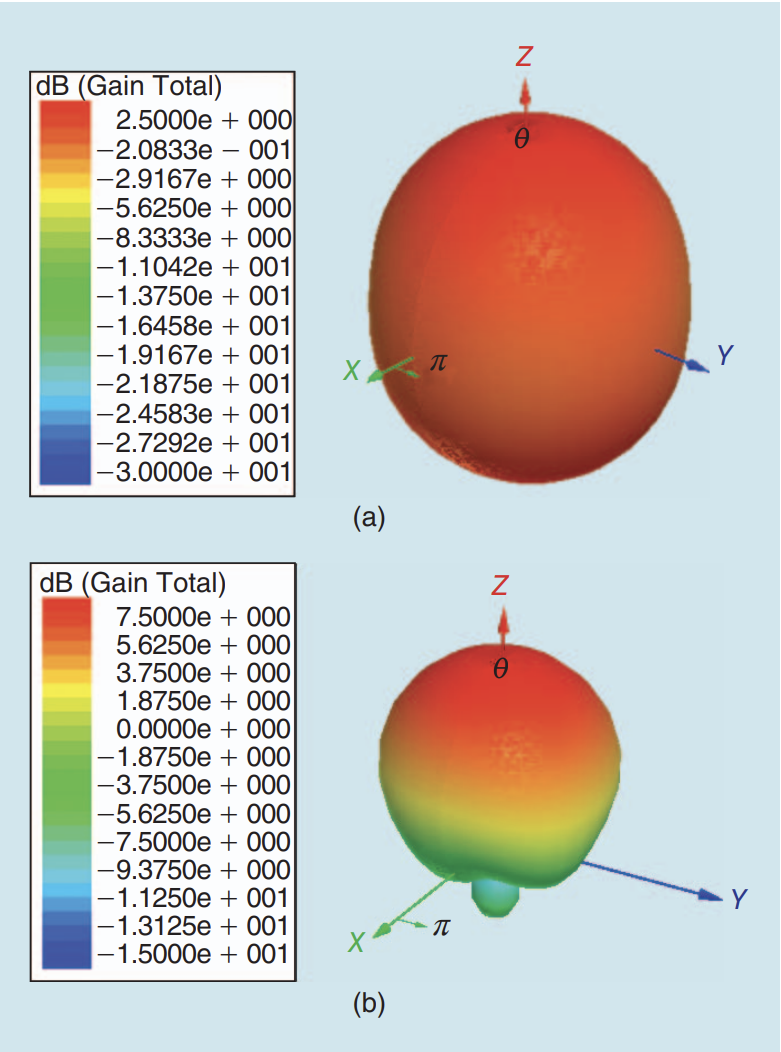
\includegraphics[width=\linewidth]{fig/crossed-dipole.png}
        \caption{Turnstile antenna radiation patterns in free space and above a finite PEC surface~\cite{ta2015crossedDipole}.}
        \label{fig:crossed-dipole}
    \end{subfigure}
    \hfill
    \begin{subfigure}[t]{0.31\linewidth}
        \centering
        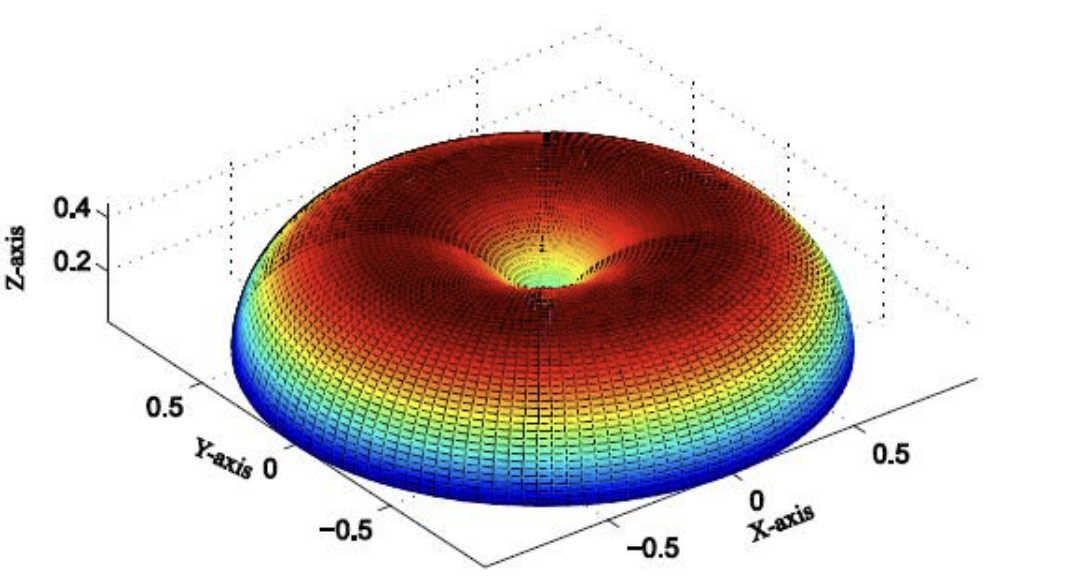
\includegraphics[width=\linewidth]{fig/Quarter wave monopole.png}
        \caption{Radiation pattern of a quarter-wave monopole above virtual ground~\cite{khan2014radiation}.}
        \label{fig:quarter-wave-monopole}
    \end{subfigure}
    \hfill
    \begin{subfigure}[t]{0.31\linewidth}
        \centering
        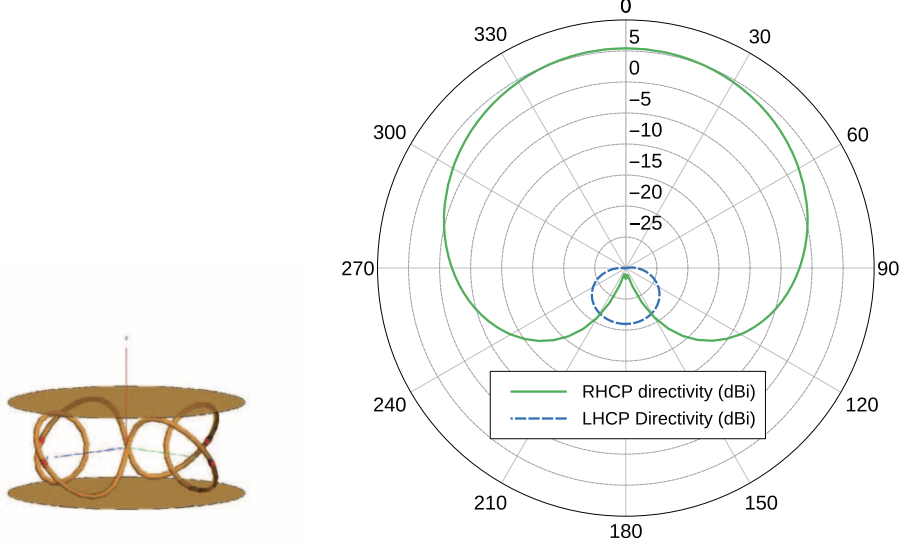
\includegraphics[width=\linewidth]{fig/ring helical.png}
        \caption{Helical-ring antenna geometry and directivity pattern~\cite{morlaas2015helical}.}
        \label{fig:helical-ring}
    \end{subfigure}
    \caption{Representative antenna concepts considered for the aerobot UHF relay link.}
    \label{fig:aerobot_antenna_concepts}
\end{figure}

Based on \autoref{tab:antenna_tradeoff}, the helical-ring/Huygens-source antenna is selected as the baseline because it provides broad hemispherical coverage, circular polarization, moderate useful gain, and low pointing sensitivity. Its main drawback is lower heritage compared with simpler dipole or monopole concepts, so additional prototyping and antenna-pattern verification are required in later design phases.
Based on \autoref{tab:antenna_tradeoff}, the helical-ring was chosen due to its performance despite having slightly lower reliability due to low heritage. 
The trade off table for the best options for the orbiter UHF antenna is shown in \autoref{tab:orbiter_UHF_antenna_tradeoff}.

\begin{table}[H]
\centering
\normalsize
\caption{Scored feasible UHF antenna type trade-off for the orbiter.}
\label{tab:orbiter_UHF_antenna_tradeoff}
\renewcommand{\arraystretch}{1.25}
\setlength{\tabcolsep}{2pt}
\resizebox{\textwidth}{!}{%
\begin{tabular}{|p{1.2cm}|p{3.0cm}|p{4.0cm}|p{3.5cm}|p{3.8cm}|p{3.7cm}|p{3.5cm}|p{3.8cm}|p{2.0cm}|}
\hline
\textbf{ID} &
\textbf{Option$\downarrow$ / Criteria$\rightarrow$} &
\textbf{Nadir Coverage / Visibility (30\%)} &
\textbf{Gain / Link Margin (20\%)} &
\textbf{Pointing Sensitivity (15\%)} &
\textbf{Polarization Performance (15\%)} &
\textbf{Mass / Integration (10\%)} &
\textbf{Reliability / Heritage (10\%)} &
\textbf{Weighted score} \\
\hline

ORB-1 &
\textbf{Quadrifilar helix} &
\cellcolor{score5!40}\textbf{5} -- Provides broad nadir-facing coverage, making it well suited for communication with an aerobot over a large part of the orbiter pass. &
\cellcolor{score4!40}\textbf{4} -- Provides low-to-moderate gain with good useful coverage; suitable for relay links where the orbiter antenna does not need to be highly directional. &
\cellcolor{score5!40}\textbf{5} -- Low pointing sensitivity due to its broad beam, while still benefiting from the orbiter's attitude control. &
\cellcolor{score5!40}\textbf{5} -- Naturally provides circular polarization, reducing polarization mismatch with a rotating or swinging aerobot antenna. &
\cellcolor{score3!40}\textbf{3} -- More bulky than a patch or simple dipole, but still practical for an orbiter-mounted UHF relay antenna. &
\cellcolor{score5!40}\textbf{5} -- Strong heritage for planetary relay communication, making it the most conservative baseline option. &
\cellcolor{score5!40}\textbf{4.60} \\
\hline

ORB-2 &
\textbf{Circularly polarized patch / patch array} &
\cellcolor{score3!40}\textbf{3} -- Provides good nadir-facing coverage, but the beam is generally more directional than a quadrifilar helix. Coverage near the edge of the pass may be weaker. &
\cellcolor{score5!40}\textbf{5} -- Can provide higher gain than a single low-gain wire antenna, especially if multiple patch elements are used. &
\cellcolor{score3!40}\textbf{3} -- Moderate pointing sensitivity; acceptable for an orbiter with attitude control, but less forgiving than a broad helical antenna. &
\cellcolor{score4!40}\textbf{4} -- Can be designed for circular polarization, giving good polarization compatibility with the aerobot link. &
\cellcolor{score5!40}\textbf{5} -- Low-profile and easy to mount on a spacecraft panel, but may require a larger surface area or array for sufficient coverage and gain. &
\cellcolor{score4!40}\textbf{4} -- Good antenna heritage in space applications, but relay coverage must be verified carefully for the required pass geometry. &
\cellcolor{score4!40}\textbf{3.85} \\
\hline

ORB-3 &
\textbf{Crossed dipole / turnstile array} &
\cellcolor{score4!40}\textbf{4} -- Can provide broad coverage if arranged properly, but the pattern depends strongly on the spacecraft mounting geometry and array configuration. &
\cellcolor{score3!40}\textbf{3} -- Low-to-moderate gain; multiple elements may be required to improve link margin or shape the nadir coverage. &
\cellcolor{score4!40}\textbf{4} -- Low pointing sensitivity if designed as a broad-beam array, but less controlled than a dedicated nadir-facing helix or patch system. &
\cellcolor{score4!40}\textbf{4} -- Can provide circular polarization if the crossed elements are fed with the correct phase relationship. &
\cellcolor{score3!40}\textbf{3} -- Lightweight elements, but array phasing, cabling, and deployment or mounting may increase integration complexity. &
\cellcolor{score3!40}\textbf{3} -- Reasonable heritage, but less straightforward as an orbiter relay antenna than a quadrifilar helix or patch design. &
\cellcolor{score4!40}\textbf{3.60} \\
\hline

ORB-4 &
\textbf{Helical-ring / Huygens-source antenna} &
\cellcolor{score4!40}\textbf{4} -- Provides broad hemispherical coverage while reducing radiation away from the desired half-space, making it conceptually attractive for nadir-facing relay communication. &
\cellcolor{score4!40}\textbf{4} -- Moderate useful gain with broad coverage; attractive if the design can be tuned to the required UHF band and spacecraft mounting geometry. &
\cellcolor{score4!40}\textbf{4} -- Low pointing sensitivity over the desired hemisphere due to its broad cardioid-like pattern. &
\cellcolor{score5!40}\textbf{5} -- Provides circular polarization over a wide angular region, which is favourable for communication with a moving or rotating aerobot. &
\cellcolor{score3!40}\textbf{3} -- Compact compared with reflector-backed solutions, but more complex to tune, feed, and qualify than conventional options. &
\cellcolor{score2!40}\textbf{2} -- Promising but lower heritage; would require mission-specific prototyping and qualification before being selected as the orbiter baseline. &
\cellcolor{score4!40}\textbf{3.85} \\
\hline

ORB-5 &
\textbf{Simple monopole / dipole} &
\cellcolor{score3!40}\textbf{3} -- Provides broad coverage, but the pattern may be strongly affected by the spacecraft body and may not be well shaped toward nadir. &
\cellcolor{score2!40}\textbf{2} -- Low gain and limited link margin; more suitable as a backup or contingency antenna than as the main relay antenna. &
\cellcolor{score3!40}\textbf{3} -- Low pointing sensitivity in some directions, but pattern nulls and spacecraft blockage can reduce performance. &
\cellcolor{score1!40}\textbf{1} -- Usually linearly polarized, causing additional loss if the aerobot antenna uses circular polarization. &
\cellcolor{score5!40}\textbf{5} -- Very simple, lightweight, and easy to integrate, especially as a backup antenna. &
\cellcolor{score4!40}\textbf{4} -- Mechanically reliable and simple, but less suitable as the primary relay antenna due to lower gain, polarization mismatch, and less controlled coverage. &
\cellcolor{score3!40}\textbf{2.80} \\
\hline

\end{tabular}%
}
\end{table}
From this trade-off, the orbiter UHF antenna had the quadrifilar helix antenna as a clear best option. For communication between earth and the Venus orbiter, a high-gain parabolic dish was chosen. This is the standard deep-space option. It provides high directivity and a high link margin for communication with Earth-based ESTRACK stations.
\subsection{link budget iterative process}
\label{subsec: link budget iterative process}
For the link budget, the end-to-end BER is approximated as the sum of the BER contributions of the individual communication links. Therefore, the BER allocation for the aerobot--orbiter link is chosen to be at least as strict as that of the orbiter--Earth link, such that the total system requirement of $\mathrm{BER} \leq 10^{-6}$ is satisfied. The aerobot--orbiter link is the most design-driving part of the communication system, since the aerobot is more constrained in mass, volume, and available transmitter power than the orbiter. The required aerobot data rate is taken as $R_b = 1500~bits/s$.

The aerobot UHF transmit antenna gain, orbiter UHF receive antenna gain, and receiver system noise temperature are taken from the previous subsystem estimates. For each candidate modulation, the number of bits per symbol, $m$, is defined. Together with the FEC code rate, $\rho$, and the roll-off factor, $\alpha$, this determines the spectral efficiency as shown in \autoref{eq:spectral_efficiency} \cite{wertz1999smad}:
\begin{equation}
    \eta = \frac{m\rho}{1+\alpha}
    \label{eq:spectral_efficiency}
\end{equation}
where $\eta$ is the spectral efficiency in $bits/s/Hz$. The required bandwidth can then be estimated from the selected bit rate and spectral efficiency.

For different required BER , the required uncoded value of $E_b/N_0$ is first determined from the modulation performance. A coding gain is then applied based on the selected FEC code rate and coding scheme. The resulting required $E_b/N_0$ is converted to the required carrier-to-noise ratio using \autoref{eq:receiver_signal_to_noise}:
\begin{equation}
    \frac{C}{N} = \frac{E_b}{N_0}\frac{R_b}{B}
    \label{eq:receiver_signal_to_noise}
\end{equation}
where $B$ is the occupied bandwidth. This required $C/N$ is then used in the link budget to determine the required aerobot transmitter power, $P_t$ using the link budget. The maximum distance and propagation losses between the aerobot and orbiter are assumed. 

\section{communication system design}
Based on \autoref{subsec: link budget iterative process}, the required RF power was evaluated for different BER and coding options and compared with available space-grade transceivers. The GAUSS high-power UHF transceiver is selected for the aerobot because it covers the required UHF relay band, supports the selected MSK/GMSK-type modulation and FEC options, and provides sufficient data-rate and RF-power margin for the \(1500~\mathrm{bit/s}\) aerobot--orbiter link.

% \begin{figure}
%     \centering
%     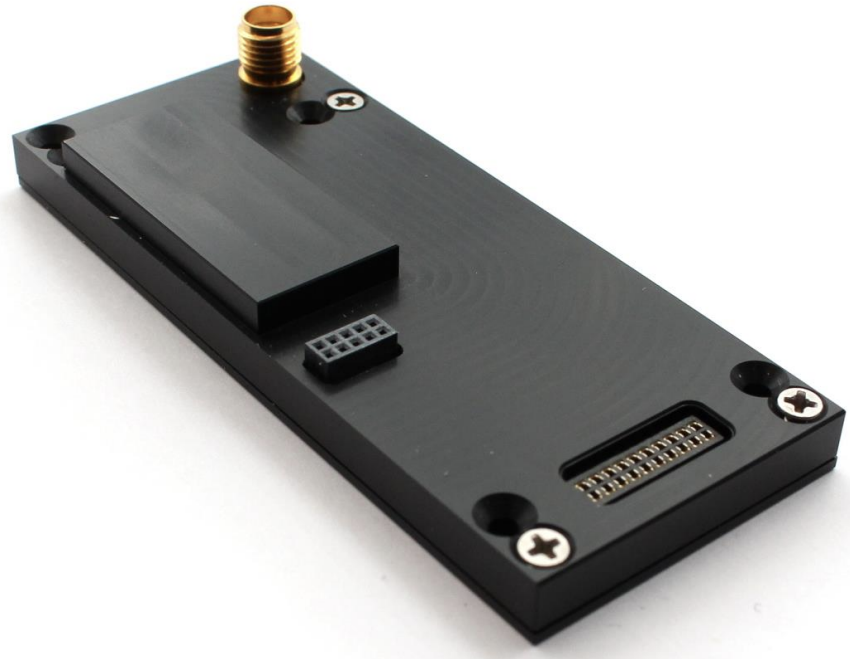
\includegraphics[width=0.2\linewidth]{fig/gauss high power transceiver.png}
%     \caption{Gauss high power transceiver}
%     \label{fig:gauss-transceiver}
% \end{figure}

\begin{table}[H]
\centering
\caption{Main GAUSS high-power UHF radio specifications.}
\label{tab:gauss_uhf_radio_specs}
\scriptsize
\renewcommand{\arraystretch}{1.10}
\setlength{\tabcolsep}{3pt}
\begin{tabular}{|p{3.5cm}|p{9.0cm}|}
\hline
\textbf{Parameter} & \textbf{Value} \\
\hline
Frequency range & RX: 390--500 MHz; TX: 400--450 MHz \\
\hline
RF output power & Software-configurable, 30--40 dBm; maximum specified value of 40.1 dBm at 400 MHz \\
\hline
Data rate & 0.3--250 kbps; current maximum stated as 100 kbps \\
\hline
Sensitivity & \(-122\) dBm at 1.2 kbps; \(-119\) dBm at 9.6 kbps; \(-109\) dBm at 50 kbps \\
\hline
RF efficiency & Typically 40--55\%, up to 59\%, depending on RF output power \\
\hline
Supported modulation / coding & FSK, MSK, GFSK, GMSK; Viterbi, Reed--Solomon FEC, and turbo coding supported \\
\hline
Supply voltage & 3.3 V digital supply and 7--12 V power-amplifier supply \\
\hline
Electrical power usage & Approximately 0.22 W in standby/reception; 17.2--19.6 W at maximum RF output with 12 V PA supply \\
\hline
Mass and size & 37 g; \(75 \times 31.5 \times 12.5~\mathrm{mm}\) \\
\hline
Temperature range & \(-40^\circ\mathrm{C}\) to \(+85^\circ\mathrm{C}\) \\
\hline
\end{tabular}
\end{table}

The orbiter requires a transponder capable of supporting both the UHF proximity relay and the X-band Earth link. The UST-Lite is selected as a representative orbiter transponder because its modular SDR architecture supports deep-space and relay communication, CCSDS-compatible operation, multiple simultaneous channels, and high-rate telemetry interfaces.

\begin{table}[H]
\centering
\caption{Main properties of the UST-Lite transponder.}
\label{tab:ust_lite_transponder_specs}
\scriptsize
\renewcommand{\arraystretch}{1.10}
\setlength{\tabcolsep}{3pt}
\begin{tabular}{|p{3.6cm}|p{8.9cm}|}
\hline
\textbf{Parameter} & \textbf{Value} \\
\hline
Supported links & Direct-to-Earth, user-terminal, and proximity relay communication using modular multi-band SDR architecture \\
\hline
Frequency bands & S, X, K, and Ka bands; UHF module possible for relay applications, assumed approximately 390--450 MHz \\
\hline
Data rates & Up to 100 Mbps; higher data rates available upon request \\
\hline
Modulation & CCSDS-compatible SDR modulation; assumed BPSK/QPSK/OQPSK, GMSK, and higher-order modes depending on configuration \\
\hline
Channel coding & CCSDS and LDPC supported; Reed--Solomon, convolutional, Turbo, and concatenated coding assumed possible from UST heritage \\
\hline
RF output power & Not specified; assumed similar to UST at approximately \(+12~\mathrm{dBm}\), with external power amplifiers required for spacecraft EIRP \\
\hline
Receiver noise figure & Not specified; assumed similar to UST: \(<3.2~\mathrm{dB}\) for S/X/Ka and \(<3.9~\mathrm{dB}\) for UHF \\
\hline
Mass and volume & \(3.4~\mathrm{kg}\) and \(113 \times 121 \times 200~\mathrm{mm}\) for a dual-band configuration; depends on selected bands \\
\hline
Power consumption & 28 V unregulated supply; approximately 35 W typical for a dual-band configuration \\
\hline
Interfaces & 10 Gbps SerDes, \(4\times\) SpaceWire, \(2\times\) JTAG, and \(3\times\) UART \\
\hline
Radiation tolerance & \(40~\mathrm{krad}\) TID; SEL immune up to \(38~\mathrm{MeV\cdot cm^2/mg}\) \\
\hline
Additional capabilities & Up to four full-duplex independent channels, expandable DSP module, clock disciplining, and ranging capability \\
\hline
\end{tabular}
\end{table}
A CCSDS-compatible rate-\(1/2\) turbo code with the 1784-bit information block is selected for all four links. From the CCSDS performance curves, this provides an effective coding gain of approximately \(10~\mathrm{dB}\), as shown in \autoref{fig:coding-gains}, at the cost of increased latency. The proximity aerobot--orbiter links use MSK modulation because its constant-envelope waveform enables efficient nonlinear power amplification and reduces transmitter power consumption. The Earth--orbiter links use BPSK because it is simple, robust at low \(E_b/N_0\), and suitable for low-data-rate deep-space communication. A roll-off factor of \(0.35\) is selected from the link-budget iteration. The final link budgets are shown in \autoref{tab:final_link_budget} and satisfy the minimum link-margin requirements of \(3~\mathrm{dB}\) for downlink and \(6~\mathrm{dB}\) for command links~\cite{chen2006linkSystemDesign}.
%coding schemes + digital modulation types
%total design block diagram
%total link budget

{\scriptsize
\renewcommand{\arraystretch}{1.12}
\setlength{\tabcolsep}{2pt}

\begin{xltabular}{\textwidth}{|
>{\raggedright\arraybackslash}p{3.1cm}|
>{\centering\arraybackslash}p{1.1cm}|
>{\raggedright\arraybackslash}X|
>{\raggedright\arraybackslash}X|
>{\raggedright\arraybackslash}X|
>{\raggedright\arraybackslash}X|}
\caption{Communication subsystem link budget summary.}
\label{tab:final_link_budget}\\

\hline
\textbf{Parameter} &
\textbf{Unit} &
\textbf{Aerobot--Orbiter Uplink} &
\textbf{Orbiter--Aerobot Downlink} &
\textbf{Earth--Orbiter Uplink} &
\textbf{Orbiter--Earth Downlink} \\
\hline
\endfirsthead

\caption[]{Communication subsystem link budget summary continued.}\\
\hline
\textbf{Parameter} &
\textbf{Unit} &
\textbf{Aerobot--Orbiter Uplink} &
\textbf{Orbiter--Aerobot Downlink} &
\textbf{Earth--Orbiter Uplink} &
\textbf{Orbiter--Earth Downlink} \\
\hline
\endhead

\hline
\multicolumn{6}{r}{\textit{Continued on next page}}\\
\endfoot

\hline
\endlastfoot

\multicolumn{6}{|l|}{\textbf{Frequency and transmitter}} \\
\hline
Frequency & MHz / GHz & 391 MHz & 401 MHz & 7.175 GHz & 8.425 GHz \\
\hline
Transmitter type & -- & Aerobot UHF transceiver & UST-Lite UHF module & ESTRACK ground station & UST-Lite X-band module + PA \\
\hline
Transmitter antenna type & -- & Helical-ring antenna & Quadrifilar helix & ESTRACK dish & High-gain parabolic dish \\
\hline
Transmitter antenna gain & dBi & 4.09 & 4.00 & 65.81 & 34.38 \\
\hline
Transmitter RF power, $P_t$ & dBW & 4.71 & 6.99 & 43.01 & 11.30 \\
\hline
Transmitter line loss & dB & 0.50 & 0.50 & 1.00 & 1.00 \\
\hline
Backoff / implementation loss at transmitter & dB & 0.00 & 0.00 & 0.00 & 0.00 \\
\hline
EIRP & dBW & 8.30 & 10.49 & 107.82 & 44.69 \\
\hline

\multicolumn{6}{|l|}{\textbf{Propagation path}} \\
\hline
Propagation range & km & 40 000 & 40 000 & 261 000 000 & 261 000 000 \\
\hline
Free-space path loss & dB & 176.32 & 176.54 & 277.89 & 279.28 \\
\hline
Atmospheric / ionospheric losses & dB & 2.50 & 2.50 & 0.50 & 0.50 \\
\hline
Scintillation / fade margin & dB & 2.00 & 2.00 & 0.00 & 0.00 \\
\hline
Pointing loss & dB & 1.50 & 1.50 & 0.70 & 0.70 \\
\hline
Polarization loss & dB & 0.00 & 0.00 & 0.20 & 0.20 \\
\hline
Combined path loss, $L_{\mathrm{comb}}$ & dB & 182.32 & 182.54 & 279.29 & 280.68 \\
\hline

\multicolumn{6}{|l|}{\textbf{Receiver}} \\
\hline
Receiver type & -- & UST-Lite UHF module & Aerobot UHF transceiver & UST-Lite X-band module & ESTRACK ground station \\
\hline
Receiver antenna type & -- & Quadrifilar helix & Helical-ring antenna & High-gain parabolic dish & ESTRACK dish \\
\hline
Receiver antenna gain & dBi & 4.00 & 4.09 & 32.99 & 67.20 \\
\hline
Receiver line loss & dB & 0.50 & 0.50 & 1.00 & 0.30 \\
\hline
Received carrier power, $C$ & dBW & -170.52 & -168.46 & -139.48 & -169.09 \\
\hline
System noise temperature, $T_s$ & dB-K & 21.76 & 24.77 & 21.76 & 13.98 \\
\hline
Receiver $G/T$ & dB/K & -18.26 & -21.18 & 10.23 & 52.92 \\
\hline
Receiver $C/N_0$ & dB-Hz & 36.32 & 35.36 & 67.36 & 45.53 \\
\hline

\multicolumn{6}{|l|}{\textbf{Data and link performance}} \\
\hline
Data rate, $R_b$ & bit/s & 1500 & 500 & 1500 & 10000 \\
\hline
Data rate, $10\log_{10}(R_b)$ & dB-Hz & 31.76 & 26.99 & 31.76 & 40.00 \\
\hline
Modulation & -- & MSK & MSK & BPSK & BPSK \\
\hline
Code type & -- & Turbo & Turbo & Turbo & Turbo \\
\hline
Code rate, $\rho$ & -- & 0.50 & 0.50 & 0.50 & 0.50 \\
\hline
Roll-off factor, $\alpha$ & -- & 0.35 & 0.35 & 0.35 & 0.35 \\
\hline
Occupied bandwidth & Hz / kHz & 4050 Hz & 1350 Hz & 4050 Hz & 27000 Hz \\
\hline
Available $E_b/N_0$ & dB & 4.56 & 8.37 & 35.60 & 5.53 \\
\hline
Required $E_b/N_0$ & dB & 1.55 & 1.55 & 2.52 & 2.52 \\
\hline
Coding gain & dB & 10.00 & 10.00 & 10.00 & 10.00 \\
\hline
Modem implementation loss & dB & 1.00 & 1.00 & 1.00 & 1.00 \\
\hline
Link margin & dB & 3.01 & 6.83 & 33.08 & 3.01 \\

\end{xltabular}
}
\autoref{tab:final_link_budget} assumes the largest expected communication distances. Although the selected UHF radios can provide up to approximately \(5~\mathrm{W}\) RF output power, the nominal link budget requires only about \(1{-}3~\mathrm{W}\). This power headroom allows operation below the maximum rating, improving thermal reliability and leaving margin for unmodelled effects such as ageing, radiation degradation, temperature-dependent amplifier performance, antenna misalignment, additional line losses, and unexpected propagation losses.




% For the two-plate helical-ring antenna, a pre-margin mass estimate of 60 g is selected. The estimate is based on the compact eight-turn HRA from Morlaas et al.~\cite{morlaas2015}, which has an outer radius of 11.14 mm, an inner radius of 5.57 mm, and a height of 5.57 mm at 1.579 GHz. Scaling this geometry to 400 MHz gives $S_f = 1.579 / 0.400 = 3.9475$, so the scaled outer radius is $R_{out} = 11.14 \cdot 3.9475 = 43.98$ mm and the scaled height is $h = 5.57 \cdot 3.9475 = 21.99$ mm. The helical conductor length is estimated as 0.592 m. For a 2.0 mm diameter copper conductor, the ring mass is $m_{ring} = 8.96 \cdot \pi \cdot (0.10)^2 \cdot 59.2 = 16.7$ g, where the density of copper is 8.96 g/cm$^3$, the wire radius is 0.10 cm, and the length is 59.2 cm. The two loading plates are taken as 0.5 mm thick aluminium disks with radius 4.398 cm, giving $m_{plates} = 2 \cdot 2.70 \cdot \pi \cdot (4.398)^2 \cdot 0.05 = 16.4$ g. An 80 mm by 80 mm by 1.0 mm RF support/feed board with two 35 micrometer copper cladding layers is estimated as $m_{board} = 8 \cdot 8 \cdot 0.10 \cdot 1.85 + 2 \cdot 8 \cdot 8 \cdot 0.0035 \cdot 8.96 = 15.9$ g. Finally, adding 7 g for the connector and feed probes and 4 g for small spacers and fasteners gives $m_{total} = 16.7 + 16.4 + 15.9 + 7 + 4 = 60.0$ g. Therefore, 60 g is used as the pre-margin mass estimate for the two-plate HRA at 390--410 MHz.
The UHF communication subsystem mass budget and peak power estimate are summarized in \autoref{tab:uhf_mass_power_budget}. The mass margins are applied according to ECSS design-margin practice~\cite{ecss2010_design_margins}, while the transmit power represents a conservative worst-case value based on the maximum aerobot--orbiter range; nominal operation is expected to require lower RF power.

\begin{table}[H]
\centering
\small
\caption{Aerobot UHF communication subsystem mass and power budget}
\label{tab:uhf_mass_power_budget}
\renewcommand{\arraystretch}{1.12}
\setlength{\tabcolsep}{4pt}
\begin{tabular}{p{4.5cm} p{3.4cm} c c c}
\hline
\textbf{Mass item} & \textbf{Dimensions / description} & \textbf{Mass [g]} & \textbf{Margin [\%]} & \textbf{Mass after margin [g]} \\
\hline
GAUSS High Power UHF Radio & \(75 \times 31.5 \times 12.5~\mathrm{mm}\) & 37.0 & 10 & 40.7 \\
Two two-plate HRA antennas & \(2 \times (\varnothing 88 \times 22~\mathrm{mm})\) & 120.0 & 20 & 144.0 \\
RF cables, connectors, antenna supports, mounting hardware, and harnessing & Routed integration hardware & 80.0 & 20 & 96.0 \\
\hline
\textbf{Total mass} & -- & \textbf{237.0} & -- & \textbf{280.7} \\
\hline
\multicolumn{5}{c}{} \\
\hline
\textbf{Power mode / item} & \textbf{Description} & \multicolumn{3}{c}{\textbf{Power [W]}} \\
\hline
Required RF output power & Worst-case link-budget value & \multicolumn{3}{c}{2.96} \\
Receive mode & Transceiver receiving only & \multicolumn{3}{c}{0.22} \\
Transmit mode & Estimated maximum operational transmit mode & \multicolumn{3}{c}{6.30} \\
Transmit + receive mode & Simultaneous transmit and receive & \multicolumn{3}{c}{6.52} \\
\hline
\end{tabular}
\end{table}
%block diagram of comms system


\section{Command and Data Handling System Design}

The C\&DH design is preliminary and will be refined once the exact payload data-generation timeline and orbiter contact windows are better known. The current design is driven by low processed payload data rates, intermittent communication, autonomous operation, and the need to store data during no-contact periods. The top-level requirements are listed in \autoref{tab:obc_cdh_requirements}.

\begin{table}[H]
\centering
\caption{Top-level C\&DH/OBC data-handling requirements}
\label{tab:obc_cdh_requirements}
\small
\renewcommand{\arraystretch}{1.15}
\begin{tabular}{p{2.2cm} p{10.8cm}}
\hline
\textbf{ID} & \textbf{Requirement} \\
\hline
REQ-CDH-01 & The C\&DH subsystem shall support an aggregate incoming telemetry rate of at least \(4~\mathrm{kbit/s}\) from payload, IMU, barometer, and housekeeping sources. \\
\hline
REQ-CDH-02 & The C\&DH subsystem shall time-tag all accepted telemetry packets with a time resolution of \(1~\mathrm{s}\) or better. \\
\hline
REQ-CDH-03 & The C\&DH subsystem shall provide at least \(32~\mathrm{MB}\) of usable non-volatile storage for science and housekeeping data. \\
\hline
REQ-CDH-04 & The C\&DH subsystem shall forward stored telemetry to the communication subsystem at a useful output rate of at least \(1500~\mathrm{bit/s}\) during nominal orbiter contact. \\
\hline
REQ-CDH-05 & The C\&DH subsystem shall preserve a protected fault-log and critical-housekeeping memory region of at least \(512~\mathrm{kB}\) during nominal operation and after processor reset. \\
\hline
REQ-CDH-06 & The C\&DH subsystem shall transmit each validated telecommand to the correct payload or subsystem interface within \(5~\mathrm{s}\) of command acceptance during nominal operation. \\
\hline
\end{tabular}
\end{table}

The theoretical storage requirement was estimated using the selected payload duty cycles, instrument data rates, a four-day day/night cycle, continuous barometer operation, and a \(20\%\) daytime orbiter contact window. Science instruments are assumed to operate only during daytime, while barometers operate continuously. Assuming the duty cycles are distributed over the daytime period, the maximum accumulated data volume is approximately \(10~\mathrm{MB}\). A practical storage requirement of \(32{-}130~\mathrm{MB}\) is therefore selected to include margin for burst measurements, packet overhead, missed contacts, and retransmissions. 

\begin{figure}[H]
    \centering
    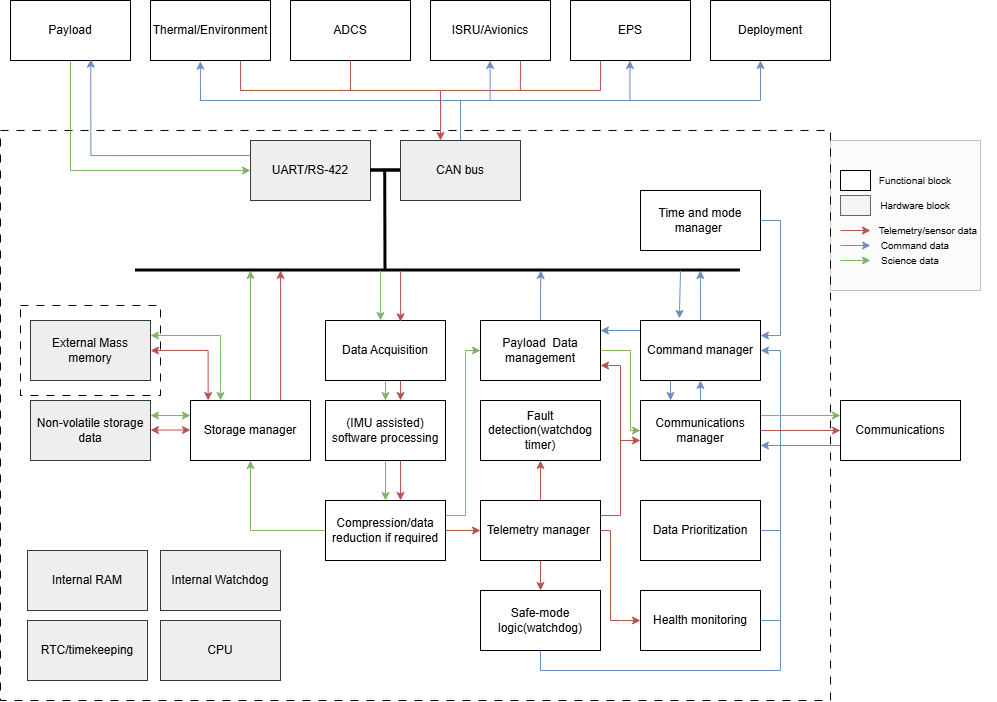
\includegraphics[width=1.0\linewidth]{fig/OBC block diagram.png}
    \caption{Data handling block diagram}
    \label{fig:OBC-block}
\end{figure}

The selected representative OBC is the Alén Space DARA OBC. It agrees with the proposed C\&DH architecture because it integrates the required processor, memory, RTC, watchdog/reset circuit, IMU, board sensors, and subsystem interfaces needed for payload scheduling, telemetry acquisition, IMU-assisted processing, storage management, command handling, health monitoring, and safe-mode recovery. The integrated \(128~\mathrm{MB}\) NAND Flash is selected as the primary science and housekeeping buffer, while the \(512~\mathrm{kB}\) MRAM is reserved for critical status and fault information.

\begin{table}[H]
\centering
\caption{Main properties of the selected DARA OBC}
\label{tab:dara_obc_properties}
\small
\renewcommand{\arraystretch}{1.12}
\begin{tabular}{p{4.0cm} p{8.5cm}}
\hline
\textbf{Property} & \textbf{Value / description} \\
\hline
Processor & ARM Cortex-M7, 32-bit CPU with FPU, up to \(280~\mathrm{MHz}\) \\
\hline
Power and supply & \(280~\mathrm{mW}\) typical, \(3.3~\mathrm{V}\) nominal supply \\
\hline
Program and working memory & \(2~\mathrm{MB}\) program Flash, \(1.4~\mathrm{MB}\) internal RAM, and \(32~\mathrm{MB}\) SDRAM \\
\hline
Persistent storage & \(512~\mathrm{kB}\) MRAM for critical status and \(128~\mathrm{MB}\) NAND Flash for science and housekeeping data \\
\hline
Optional storage & \(2\times\) microSD card slots, up to \(64~\mathrm{GB}\) each \\
\hline
Integrated sensors & IMU with 3-axis magnetometer, gyroscope, and accelerometer; board voltage, current, and temperature sensors \\
\hline
Interfaces & \(3\times\) RS422, \(2\times\) CAN, UART, \(2\times\) I\(^2\)C, SPI, GPIO, ADC, PWM, PPS, and JTAG \\
\hline
Fault recovery and timekeeping & Hardware watchdog/reset circuit and RTC with independent power supply option \\
\hline
Environment, mass, and size & \(-40^\circ\mathrm{C}\) to \(+85^\circ\mathrm{C}\), \(115~\mathrm{g}\), \(93.3 \times 89.3 \times 12.6~\mathrm{mm}\) \\
\hline
\end{tabular}
\end{table}

\section{Sensitivity Analysis}

The design is mainly driven by the aerobot--orbiter communication link budget. Antenna selection affects gain, coverage, pointing loss, and polarization loss, while lower operating frequency reduces free-space path loss but increases antenna size and mass. A stricter BER requirement increases the required \(E_b/N_0\), reducing link margin. Data rate is also critical: since \(E_b/N_0 = C/N_0 - 10\log_{10}(R_b)\), doubling the bit rate reduces the link margin by approximately \(3~\mathrm{dB}\) if all other parameters remain unchanged. The link-budget tool was checked against these expected sensitivities.

The OBC data-handling design is most sensitive to payload data rate, duty cycle, and orbiter contact duration. Higher data generation or shorter contact time increases stored data volume and may prevent the buffer from fully emptying during a pass. However, the selected \(128~\mathrm{MB}\) NAND Flash provides significant margin above the theoretical \(10~\mathrm{MB}\) requirement. The most important parameters to refine later are therefore the real payload operation schedule and orbiter visibility duration.

\section{Verification and Validation}

Verification confirms that the communication and C\&DH designs meet their requirements, while validation confirms suitability for the Venus aerobot mission concept. The communication design tool is verified through sensitivity checks on transmitter power, antenna gain, losses, and data rate, including the relation \(E_b/N_0 = C/N_0 - 10\log_{10}(R_b)\), supporting REQ-COM-04. REQ-COM-01 and REQ-COM-02 are verified through representative transceiver tests under worst-case attenuation, measuring BER and useful data rate. REQ-COM-03 is verified by inspection of frequency band, modulation, coding, and ESTRACK compatibility. REQ-COM-05 is verified through antenna radiation-pattern measurements, orbiter-pass coverage simulation, and environmental testing.

The C\&DH requirements are verified through functional OBC tests. Representative payload, IMU, barometer, and housekeeping data streams verify REQ-CDH-01 and REQ-CDH-02 by checking accepted input rate and time-tagging. REQ-CDH-03 is verified by memory inspection and simulated day/night buffer testing, while REQ-CDH-04 is verified by forwarding stored telemetry to the communication subsystem at \(1500~\mathrm{bit/s}\). REQ-CDH-05 is verified through reset and fault-log tests, and REQ-CDH-06 through command-injection tests that confirm correct routing within the required time.

Validation is performed using mission-level scenarios. The communication subsystem is validated with a representative aerobot--orbiter relay scenario using the selected data rate, modulation, coding, contact duration, and telemetry packets. The OBC is validated through an end-to-end operational scenario including daytime payload duty cycles, continuous barometer operation, no nighttime contact, limited daytime orbiter contact, realistic data streams, and command updates. Successful validation shows that the combined communication and C\&DH design supports autonomous operation, data storage, downlink during contact windows, critical-data preservation, and safe-mode recovery.